\chapter{Technical Background}

In this chapter we present the technical background of the concepts and
protocols that are central for this thesis. We first give a introduction to
computer networks in general and how they are organized. Next, we discuss common
Web services used for exchanging data in military systems. Then we look into a
number of protocols that we can replace HTTP/TCP with in order to increase the
performance of Web services. Finally, we present some available frameworks and
solutions for creating a proxy.



\section{Network layers}

To reduce design complexity, networks are organized into layers, each one built
upon the one below it. In the Internet Protocol Suite\cite{rfc-1122}, networks
is divided into 4 layers. As stated in the scope of this thesis, we only look
into optimization techniques for the application and transport layer.

%%%%%%%%%%%% Internet Protocol Suite %%%%%%%%%%%%%%%%%%%
\begin{table}[h]
\begin{tabularx}{\textwidth}{| X |}
\hline
  \textbf{Application Layer} \\ \hline
  \textbf{Transport Layer} \\ \hline
  \textbf{Internet Layer} \\ \hline
  \textbf{Link layer} \\ \hline
\end{tabularx}
\caption{The layers of the Internet Protocol Suite}
\label{figure-network-layers}
\end{table}

\paragraph{Link layer}

The lowest layer is the link layer, where link refers to the to the physical
network component used to interconnect nodes in a network. Link layer protocols
operate between adjacent network nodes. An example of a link layer protocol is
Ethernet.

\paragraph{Internet Layer}

 Where the link layer is only concerned of moving data over a wire to an
 adjacent node, the Internet layer is concerned of how to deliver data all the
 way from a source to a destination, possible passing through multiple nodes on
 its way. It does not guarantee delivery of data, since data can be lost on the
 way to the destination. Guaranteed delivery is usually handled on the higher
 levels of the Internet Protocol Suite.

 The core protocol of the Internet layer is \gls{ip} and its routing function
 enables sending data over interconnected networks.

\paragraph{Transport layer}

In the Internet protocol suite model, the transport layer provides end-to-end
communication services for applications. It builds on top on the network layer,
and takes responsibility of sending data all the way from a process on a source
machine to a process on the destination machine. The far most used transport
protocol is the \gls{tcp}, which provides reliable transport of data to
applications. With reliable transport we mean that if data in transmission is
lost or received in the wrong order, this is all handled by the transport
protocol. This provides an important abstraction for applications so that they
don't need to deal with the characteristics of the physical network itself.

\paragraph{Application layer}

The top layer is the application layer and is where applications real user use
reside. The other layers provide transport services to applications found in the
application layer. When we talk about application layer protocols, we talk about
protocols that applications use to communicate with other applications.
Application layer protocols use the communication services the transport layer
provides.  Examples of application layer protocols is \gls{http} and \gls{ftp}.

%%%%%%% WEB SERVICES
\section{Web services}
\label{web-services}
%TO-DO lede inn smooth mot soa.
Web services are client and server applications that communicate over a
network and can be used to implement a service oriented architecture. Web
services are critical in any data systems and are in widespread use in both
civilian and military systems. It is a broad term and can be used to describe
different types of services that are available over a network. The most common
usage of the term refers to the \gls{w3c} definition of SOAP-based Web
services, but could also refer to more simple HTTP-based \gls{rest} services.

In this thesis we investigate optimization techniques that should support both
\gls{w3c} Web services and \gls{rest}ful web services.

\subsection{W3C Web services}

\gls{w3c} has defined Web services as \cite{wrc-web-service}:

\paragraph{}
\textit{
    A Web service is a software system designed to support interoperable
    machine-to-machine interaction over a network. It has an interface described in
    a machine-processable format (specifically WSDL). Other systems interact with
    the Web service in a manner prescribed by its description using SOAP-messages,
    typically conveyed using HTTP with an XML serialization in conjunction with
    other Web-related standards.
}

\paragraph{}

This definition points out a set of standards that enables machine-to-machine
interactions. All communication is based on sending XML-based SOAP messages. It
exists many definitions of Web services where the core principles are the same,
but the finer details may vary. The Web service technology is realization of the
\gls{soa} principles, which provides loose coupling and ease integration between
systems.

\begin{figure}[h]
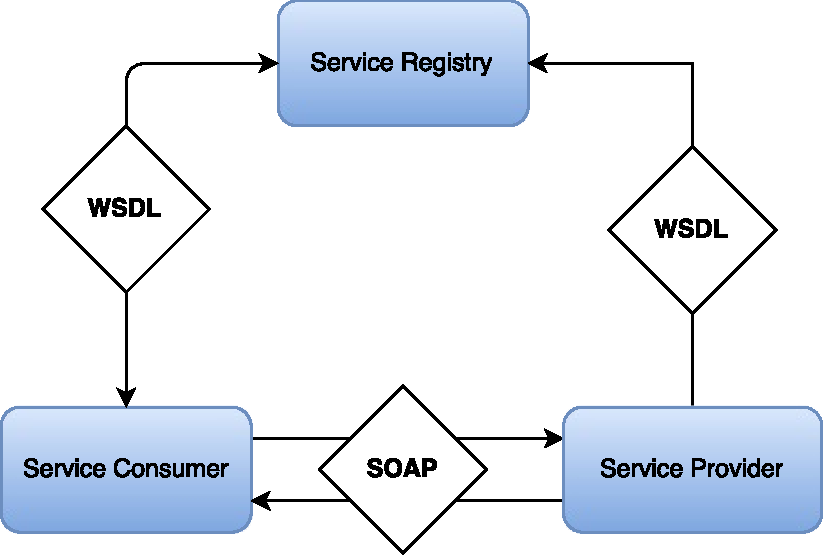
\includegraphics[scale=0.6]{images/web_services.pdf}
\caption{W3C Web services}
\label{figure-w3c-web-services}
\end{figure}

These standards that together makes W3C Web services are presented in the
following sections.

\subsubsection{XML}

The \gls{xml}\cite{W3C-XML} is considered as the base standard for Web services.
An XML document consist of data surrounded by tags and is designed to be both
machine and user readable. Tags describe the data they enclose. The tags can be
standardized, which allows exchange and understanding of data in a standardized,
machine-readable way.


\subsubsection{Service descriptions: WSDL}

\gls{wsdl} is an XML-based interface definition language that describes
functionality offered by a Web service\cite{w3c-wsdl}. The interface describes
available functions, data types for message requests and responses, binding
information about the transport protocol, as well as address information for
locating the service. This enables a formal, machine-readable description of Web
service which clients can invoke.

\subsubsection{SOAP}

SOAP is an application level, XML-based protocol specification for information
exchange\cite{w3c-soap} in the implementation of Web services. Data
communication in SOAP is done by nodes sending each other whats called SOAP
messages. A SOAP message can be considered as an "envelope" consisting of an
optional message header and a required message body. The header can contain
information not directly related to the message such as routing information for
the message and security information. The body contains the data being sent,
known as the payload.

It is transport protocol agnostic, which means it can be carried over various
underlying protocols. The far most used transport protocol is HTTP over TCP, but
other protocols such as UDP and SMTP can be used as well.

\subsection{\glsentrylong{rest}}
\label{rest}

In the previous sections we looked into the standards and specifications that
compose W3C Web services. However, there also exist other types of Web services
which does not follow the these standards. In year 2000, the computer scientist
Roy Fielding introduced \gls{rest} where he presented a model of how the web
\textit{should} work. This idealized model of interactions within an Web
application\cite{rest-fielding} is what we refer to as the REST architectural
style. REST attempts to minimize latency and network communication while
maximizing the independence and scalability of component implementations. This
is done by placing constraints on connector semantics rather than on component
semantics like W3C Web services.  REST is based on a client-server model where a
client requests data from a server when needed. While W3C Web services is
service oriented, we can look at REST as being more data oriented.

Web services that adhere to the REST style is called RESTful Web services. They
are closely associated with HTTP and use HTTP verbs(e.g GET, POST, DELETE) to
operate on information located on a server. RESTful Web services typically
expose some sort of information, called resources in REST. Resources are
identified by a resource identifier. \Cref{table-rest} illustrates how a
component exposes a set of operations of the car resource.

 %%%%%%%%%%%% REST eksempel %%%%%%%%%%%%%%%%%%%
 \begin{table}[h]
 \begin{tabularx}{\textwidth}{| X | X | X |}
 \hline
   \textbf{Resource identifier} & \textbf{HTTP Method}  & \textbf{Meaning}\\ \hline
   /vehicles/cars/1234 & GET & Return a car with ID 1234 from the system. \\ \hline
   /vehicles/cars/ & POST & Create a new car which will be added to the list of cars. \\ \hline
   /vehicles/cars/1234 & DELETE & Delete a car with ID 1234 from the system. \\ \hline
 \end{tabularx}
 \caption{Example of REST operations}
 \label{table-rest}
 \end{table}

 \gls{rest} is easy to understand and has gained a lot of traction in the civil
 industry in the latest years. Although NATO has chosen W3C Web services as the
 technology to do information-exchange, REST is identified as a technology of
 interest to certain groups in
 NATO\cite{johnsen-bloebaum-recommendations-web-services-tactical-domain}. One
 downside to NATO with REST is that it lack standardization, which may cause
 interoperability issues.

 In the next section we will look into \gls{http}, which is closely associated
 with REST and is the most used transport protocol for W3C Web services.

\section{\glsentrylong{http}}

As we have seen in the previous sections, both RESTful and W3C Web services
utilizes the \gls{http} as their way to communicate with other services. The
usage of \gls{http} is very widespread and it is the foundation of data
communication for the \glsentrylong{www} since the early 90's. It's protocol
specification is coordinated by \gls{ietf} and the \gls{w3c}, and is defined
as\cite{rfc-2616}:

\paragraph{}
\textit{
    The Hypertext Transfer Protocol (HTTP) is an application-level
    protocol for distributed, collaborative, hypermedia information
    systems. It is a generic, stateless, protocol which can be used for
    many tasks beyond its use for hypertext, such as name servers and
    distributed object management systems, through extension of its
    request methods, error codes and headers
}

\paragraph{}

\gls{http} started out as a simple protocol for raw data transfer across the
Internet and has since been updated in HTTP/1.0, HTTP/1.1 and most recently a
major update with HTTP/2.0. It is a request-reply protocol which means that all
data exchanges is initiated with a client invoking a HTTP-request and then waits
until a server responds with a HTTP response. A HTTP-request consist of the
request method, URI, protocol version, client information, and a optional body.
The server responds with a message containing a status line, protocol version, a
code indicating the success or error of the request, and a optional body. Both
HTTP requests and responses use a generic message format and can contain zero or
more HTTP headers. Headers are used to provide information about the
request/reply or about the message body, e.g information about the encoding and
caching information.

HTTP, being an application level protocol, relies on a transport protocol to
actually transfer data to an another machine. HTTP communication most often, but
not necessarily, occurs over TCP/IP connections. The only requirement in HTTP
specification is that a reliable transport protocol is used.

\subsubsection{HTTP methods}

 Associated with all HTTP requests are a request method, which indicates the
 desired action to be performed on a resource located on a Web server. The set
 of HTTP methods defined in HTTP/1.1 is listed in \cref{table-http-methods}.

 %%%%%%%%%%%% HTTP methods %%%%%%%%%%%%%%%%%%%
 \begin{table}[h]
 \begin{tabularx}{\textwidth}{| X | X |}
 \hline
   \textbf{HTTP Method} & \textbf{Purpose} \\ \hline
   OPTIONS & Asks the server which HTTP methods and header field it supports. \\ \hline
   GET & Retrieve information identified by the resource indentifier(Request-URI). \\ \hline
   HEAD & Identical to GET, except that the HTTP-body is not returned from the server. \\ \hline
   POST & Asks the server to accept the message payload from the client as a new resource.\\ \hline
   PUT & Similar to POST but allows the client to ask the server to update a resource identified by the request-uri \\ \hline
   DELETE & Requests that the resource identified by the request-uri is deleted \\ \hline
   TRACE & Echoes the HTTP request. Used for debugging \\ \hline
   CONNECT & For use with a proxy that can dynamically switch to being a tunnel\\ \hline
 \end{tabularx}
 \caption{HTTP methods}
 \label{table-http-methods}
 \end{table}

\section{\glsentrylong{tcp}}
\label{tcp}

\gls{tcp} is called the workhorse of the Internet because it is so critical for
how the Internet works. It is the primary transport protocol of the Internet
Protocol Suite\cite{rfc-1122} and provides reliable, in-sequence delivery of
two-way traffic(full-duplex) data. HTTP most often uses TCP as its transport
protocol. In this subsection we present the characteristics of TCP and some of
the issues we may encounter working with it.

\gls{tcp} was defined in RFC 793\cite{rfc-793} back in September 1981 and has
since been improved in various RFC's. The main motivation behind \gls{tcp} was
to provide reliable end-to-end byte streams over unreliable networks.

\paragraph{Reliablility}

When transferring data over the Internet, the data may pass through various
networks, routers and physical networks. Some of the routers may be not working
correctly, a bit may be flipped when transferring data wirelessly, or some other
factor may come in to play. For those reasons, we have to accept that some of
the data will be damaged, lost, duplicated or delivered out of order.

TCP recovers from such faults by assigning sequence number to each packet being
sent. It then requires an positive acknowledgement from the receiver that the
data was actually received. If the acknowledgement is not received within a
timeout interval, the data is transmitted again. For the receiver the sequence
numbers are used to ensure that data is received in the correct order, as well
as eliminating duplicates. Furthermore, to detect damaged data, TCP applies
checksums to each segment transmitted. At the receiver the checksum is then
checked and damaged segments are discarded.

\paragraph{Flow Control}

If a fast receiver sends data faster than a slow receiver is able to process,
the receiver will be swamped with data and may experience serious performance
reduction. Flow control is a mechanism to manage the rate of the data
transmission to avoid overflowing a receiver. TCP provides this by using a
window of acceptable sequence numbers that the receiver is willing to accept.
With every acknowledgement sent back to the sender, the window is specified.
This allows the receiver to control which segments, and how fast, the sender
can send.

\paragraph{Connection}

TCP is connection-oriented, which means that a connection between a sender and
the receiver must be established before any data can be transfered. A connection
is specified by a pair of sockets identifying its two sides. Associated with
each connection TCP initialize and maintains some status information for each
connection. This includes window size, socket information and sequence numbers.

\paragraph{Protocol}

Computers supporting TCP has a piece of software, which manages TCP streams and
interfaces to the IP layer. Most often this software is a part of the
kernel\cite{computer-networks}. It accepts data streams from local processes,
and breaks them up into pieces, before sending them to the IP layer. The pieces
are called TCP segments, which consist of a fixed 20 byte header, followed by
zero or more data byte. The TCP software decide how big the segment should be,
but for performance reasons they should not exceed the \gls{mtu} of the
link(the physical network). Each segment should be so small that they can be
sent in a single, unfragmented package over the entire network. This usually
limits the size of each segment to the \gls{mtu} of the Ethernet, which is 1500
bytes.

When the TCP software receives data from applications, it is not necessarily
sent immediately as it may be buffered before its sent. At the receiver, data is
delivered to the TCP software, which reconstructs the original byte streams and
deliver them to the target application.


\section{Protocols of interest}

% Trengs en diskjon om NATO's everything over IP her. Man sier det i scope, men
%må diskutere det her.

Since previous experiments have shown that employing Web services built on
HTTP/TCP breaks down in networks with the DIL characteristics, we're in this
thesis looking into alternative protocols. One important limitation however, is
that NATO has chosen the "everything over IP", which means that all optimization
must ocour on the top of the network layer. Of this follows that we will
evaluate protocols in the transport and application layer of the Internet
Protocol Suite.

In the following sections we will give a short introduction to the protocols
we're investigating in this thesis. We'll get started by discussing \gls{udp},
which alongside \gls{tcp} is one of the core protocols of the Internet protocol
suite. The remaining protocols discussed in the next section all use either
\gls{tcp} or \gls{udp} as their transport protocol.

Skrive noe om hvorfor vi har valgt de protokollene som vi velger å presentere i denne seksjonen.

\subsection{\glsentrylong{udp}}

The Internet has two main protocols in transport layer, \gls{udp} and \gls{tcp}.
They have fundamentally different characteristics and use cases, which we will
go through in this section. \gls{udp} was formally defined in 1980 in RFC
768\cite{rfc-udp} and is a more simpler protocol than \gls{tcp}. It sends
messages, called datagrams, to nodes over the \gls{ip} network. While \gls{tcp}
provides reliable transmission along with flow control and congestion control,
does UDP only support sending IP datagrams. Furthermore it is a connectionless
protocol, which means that the protocol can send messages \textit{without} first
establishing a connection. Since \gls{udp} does not provide guaranteed delivery
or in-order delivery of messages, it should only be used by applications that
does not require this.

To summarize, \gls{udp} is a more lightweight protocol than TCP. It has smaller headers and
less overhead, which makes it faster protocol. The downside is that is does not
provide any mechisms for reliability. However, it is worth to note that
applications can build their own reliability on top of \gls{udp}.

\subsection{\glsentrylong{coap}}

\gls{coap} is a specialized Web transfer protocol standardized in June 2014
designed for use with constrained nodes and  networks\cite{rfc-7252}. It is
designed for machine-to-machine applications, typically in the Internet of
Things. Furthermore it is designed with an similar interface as HTTP, in order
to easily integrate with Web services. \gls{coap} is based on the REST model,
where the server makes resources available  under a resource identifier(URI).
Clients access these resources using the HTTP-verbs GET, PUT, POST and DELETE.
CoAP main features includes:

\begin{itemize}

    \item UDP transport with optional reliability supporting unicast and
    multicast requests.

    \item Asynchronous message exchanges.

    \item A stateless HTTP mapping, allowing proxies to be built providing
    access to CoAP resources via HTTP in a uniform way or for HTTP simple
    interfaces to be realized alternatively over CoAP.

     \item Low header overhead and parsing complexity.

\end{itemize}

\gls{coap} works similar to HTTP in the way that they use a client-server
interaction model. \gls{coap} requests is sent from a client to request an
action on a resource located on a server. The server then responds with a
response code and a possible response body. Unlike HTTP which uses TCP as its
transport protocol, \gls{coap} uses \gls{udp}. Since \gls{udp} does not
guarantee delivery, \gls{coap} provide mechanisms for optional reliability.

\begin{figure}[h]
\centering
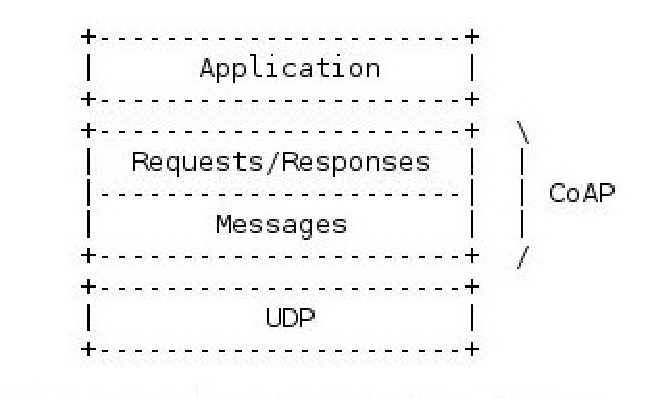
\includegraphics[scale=0.6]{images/coap.pdf}
\caption{Overview of CoAP}
\end{figure}


\subsection{\glsentrylong{amqp}}

\gls{amqp} is a messaging middleware that can utilize different transport
protocols.

\begin{itemize}
    \item Support both request/response and publish/subscribe communication
    paradigms.
    \item Reliable when facing network disruptions, since it employs a
    broker-based architecture with store-and-forward capabilities.
\end{itemize}

\subsection{\glsentrylong{mqtt}}

MQTT is a client server publish/subscribe messaging transport protocol
\cite{oasis-mqtt}. It is considered lightweight and is designed for use in networks
where the bandwidth is limited. It is broker-based, where the broker is
responsible for delivering messages to clients based on the topic of a
message.

\subsection{\glsentrylong{sctp}}

\gls{sctp} is transport-layer protocol, which offers functionality from both \gls{udp} and \gls{tcp}.
\begin{itemize}
    \item Message-oriented like UDP.
    \item Ensure reliable, in sequence transport of messages with congestion control like TCP.
    \item Multi-homing and multi-streaming.
\end{itemize}





\section{Proxies}

A proxy is an application which acts as an intermediary between an client and a
server. Proxies are widely in use and their usage and type varies. Example of
usage is load balancing, caching and security. Web proxies are proxies that
forward HTTP requests, which is what we are investigating in this thesis.

In this section we will briefly present available popular web proxies.

\subsection{Apache}

\subsection{Squid}

\subsection{Apache Camel}

This does the work of converting the specific input/request (like an HTTP
request) into something generic - a Camel Exchange - that can travel down a
Route.
 - quoute. må skrives om.

\subsection{Nginx}


\section{Performance testing}

To determine which optimization techniques that have a positive effect on the
performance of Web services in DIL environments, we can do performance testing.

\subsection{Network metrics}

Network metrics are used to describe various aspects of data transfer from a
point to another.

\begin{description}

\item[Link throughput] The link throughput is influenced by how large distance
there is between the units communicating.

\item[Link reliability] How much of the arriving data that is correct. This is
called \textit{bit error rate} or \textit{packet error rate}. With high error
rates, more data to be transmitted again due to the data arriving being
incorrect. This contributes to longer transmission time. In a military setting,
an enemy may deliberate sabotage the network with jamming, causing higher error
rates.

\item[Link latency] The communication technology in use influences how fast data
transmission can be done. Long delay may cause that the application sending data
timing out.

\end{description}

\section{Summary}
Summary of background chapter here.

%%%%%%%%%%%% Transport protokoller %%%%%%%%%%%%%%%%%%%
\begin{table}[h]
\begin{tabularx}{\textwidth}{| X | X |}
\hline
  \textbf{Protocol} & \textbf{Summary} \\ \hline
  HTTP over TCP & Widely used. Breaks down in DIL environments.\\ \hline
  CoAP & Application level protocol designed for use in the Internet of Things. \\ \hline
  AMQP & Messaging middleware with store-and-forward capabilities.\\ \hline
  MQTT & Summary here\\ \hline
  SCTP & Similar to UDP but also provide reliable, in sequence transport of messages like TCP. \\ \hline
  TCP & The well-known transport protocol. \\ \hline
  UDP & Lacks reliability, but frameworks exist that provides it. \\ \hline
\end{tabularx}
\caption{Protocols of Interest}
\end{table}
